\documentclass[11pt,a4paper]{article}
\usepackage[utf8]{inputenc}
\usepackage{amsmath}
\usepackage{graphicx}
\usepackage{hyperref}
\usepackage{booktabs}
\usepackage{geometry}
\geometry{margin=1in}

\title{\textbf{Memory Economics: Environmental Volatility Selects Between Lamarckian Inheritance and Agile Amnesia}}
\author{\textbf{Prince T Philip} \\ \texttt{princephilip514@gmail.com}}
\date{October 10, 2026}

\begin{document}
\maketitle

\begin{abstract}
In generational artificial life models, the optimal rate of knowledge inheritance is classically assumed to be bounded monotonically by the rate of environmental change. We show that when learning speed and memory capacity co-evolve alongside retention rates under metabolic constraints, the evolutionary dynamics of memory become highly non-monotonic. We map the trade-off surface of retention ($f$), learning rate ($lr$), and capacity ($c$) across a spectrum of environmental shift frequencies. Extremely rapid environmental fluctuation (shifts every 2 generations) produces a ``boomerang'' strategy favoring larger brain capacity ($c \approx 1.04 \pm 0.25$), reduced learning rates ($lr \approx 0.035 \pm 0.018$), and elevated retention ($f \approx 0.55 \pm 0.34$), as retaining old skills is metabolically cheaper than repeatedly relearning them. Intermediate volatility flips the population into ``agile amnesia,'' characterized by low retention ($f \approx 0.21 \pm 0.07$), elevated learning rates ($lr \approx 0.054 \pm 0.004$), and smaller capacities ($c \approx 0.74 \pm 0.06$). Long-term environmental stability selects for ``Lamarckian rentiers'' exhibiting high retention ($f > 0.80$) and minimal learning. Furthermore, tracking information provenance reveals that in the agile amnesia regime, up to 85.6\% of active memory consists of newly acquired data, relegating inherited knowledge to a short-lived bootstrap buffer. These findings reframe biological and artificial inheritance as fluid economic equilibria governed by environmental cadence and the metabolic costs of neuroplasticity.
\end{abstract}

\section{Introduction}
A fundamental challenge for adaptive systems in non-stationary environments is balancing the retention of ancestral knowledge with the acquisition of novel skills. Previous work in this domain established that under fixed, slow learning rates and chaotic environmental shifts, evolutionary algorithms discover an optimal fractional retention rate near the Golden Ratio conjugate ($1/\phi \approx 0.618$).

However, biological agents operate under metabolic constraints where rapid learning and large memory capacities are energetically costly. This study investigates the conditional nature of that attractor. We hypothesize that optimal knowledge transmission is a function of ``memory economics'': the metabolic cost of learning, the upkeep cost of memory capacity, and the frequency of environmental change. By co-evolving retention, learning rate, and capacity, we map the full phase diagram of evolutionary strategies across multiple temporal scales of environmental volatility.

\section{Model}
We extend the Generational Artificial Life (GAL) framework to support the joint evolution of three continuous traits:
\begin{enumerate}
    \item \textbf{Retention ($f \in [0, 1]$):} The fraction of parental accumulated skill passed to offspring.
    \item \textbf{Learning Rate ($lr \in [0.001, 0.25]$):} The rate at which the agent acquires skill points during active learning.
    \item \textbf{Capacity ($c \in [0.1, 5.0]$):} The maximum total skill points an agent can hold simultaneously. If exceeded, existing skills are proportionally scaled down.
\end{enumerate}

\paragraph{Skill Accumulation and Work.}
During their lifetime, agents dedicate time steps to learning the currently active environmental skill, followed by a work phase where they attempt tasks based on their skill level.

\paragraph{Metabolic Costs.}
To reflect realistic biological trade-offs, we impose two critical costs:
\begin{itemize}
    \item \textit{Cost of Learning:} High learning rates incur a time penalty, proportionally reducing the number of tasks an agent can attempt during its work phase (simulating time spent learning rather than exploiting).
    \item \textit{Cost of Capacity:} Agents pay a baseline fitness penalty for maintaining larger memory capacities ($0.05 \times c$), regardless of whether the capacity is actively utilized.
\end{itemize}

\paragraph{Environmental Shifts and Selection.}
The environment demands one of two distinct skills ($A$ or $B$). The active skill shifts according to discrete generation schedules: Periodic (every $k$ generations) or Chaotic (intervals following Fibonacci and Pi digit sequences). Fitness reflects task success efficiency and absolute productivity, minus metabolic costs. The top 50\% of the population reproduces with Gaussian mutation applied to all three traits.

\section{Results}

\subsection{The Cost of Learning and Agile Amnesia}
Baseline experiments allowing free (zero-cost) learning resulted in an immediate crash of retention ($f \approx 0.23$) and maximized learning rates ($lr \approx 0.20$). However, introducing a moderate time penalty on learning completely reversed this dynamic, collapsing the learning rate to near-zero ($lr \approx 0.01$) and restoring high retention ($f > 0.70$). This suggests that under our model's assumptions, the ``fast-learning amnesiac'' strategy is only viable when the cost of learning is negligible; under metabolic constraints, populations revert to strict Lamarckian copying.

\subsection{Evolutionary Shrinkage of Brain Capacity}
When brain capacity ($c$) co-evolved alongside $f$ and $lr$ under chaotic environmental shifts, evolution selected for smaller brains. Mean capacity shrank from an initial 1.18 to 0.57. Because large memory is expensive to maintain and difficult to fill usefully before a chaotic shift renders it obsolete, evolutionary selection favored small, overwrite-friendly brains paired with high learning rates and low retention.

\subsection{Information Provenance}
By tracking the exact information bits utilized by agents at the end of their lifetime, we quantified the actual utilization of parental memory. In populations evolving the ``agile amnesia'' trait cluster, 85.6\% of the final skill level consisted of information actively learned during the agent's lifetime. Inherited information (14.4\%) served merely as a short-lived bootstrap buffer to survive early-life tasks before being overwritten by new learning.

\subsection{Joint Evolution Phase Diagram}
Sweeping the joint evolution across various periodic environmental shift frequencies over 5 independent seeds yields the phase diagram summarized in Table~\ref{tab:phase_diagram} and Figure~\ref{fig:phase_diagram}.

\begin{table}[h]
\centering
\caption{Final Trait Values vs. Environmental Shift Frequency (5 Seeds, Mean $\pm$ StdDev)}
\label{tab:phase_diagram}
\vspace{0.2cm}
\begin{tabular}{lcccc}
\toprule
\textbf{Environment} & \textbf{Shift Freq} & \textbf{Retention ($f$)} & \textbf{Learn Rate ($lr$)} & \textbf{Capacity ($c$)} \\
\midrule
Hyper-Volatile       & 2 gens  & $0.554 \pm 0.344$ & $0.035 \pm 0.018$ & $1.041 \pm 0.251$ \\
Highly Volatile      & 5 gens  & $0.212 \pm 0.073$ & $0.054 \pm 0.004$ & $0.739 \pm 0.056$ \\
Chaotic (Fib/Pi)     & Mixed   & $0.880 \pm 0.032$ & $0.018 \pm 0.001$ & $0.718 \pm 0.076$ \\
Moderately Volatile  & 20 gens & $0.797 \pm 0.046$ & $0.017 \pm 0.002$ & $0.697 \pm 0.053$ \\
Stable               & 50 gens & $0.835 \pm 0.040$ & $0.019 \pm 0.005$ & $0.707 \pm 0.055$ \\
Hyper-Stable         & 200 gens& $0.852 \pm 0.037$ & $0.015 \pm 0.003$ & $0.658 \pm 0.067$ \\
\bottomrule
\end{tabular}
\end{table}

\begin{figure}[htbp]
\centering
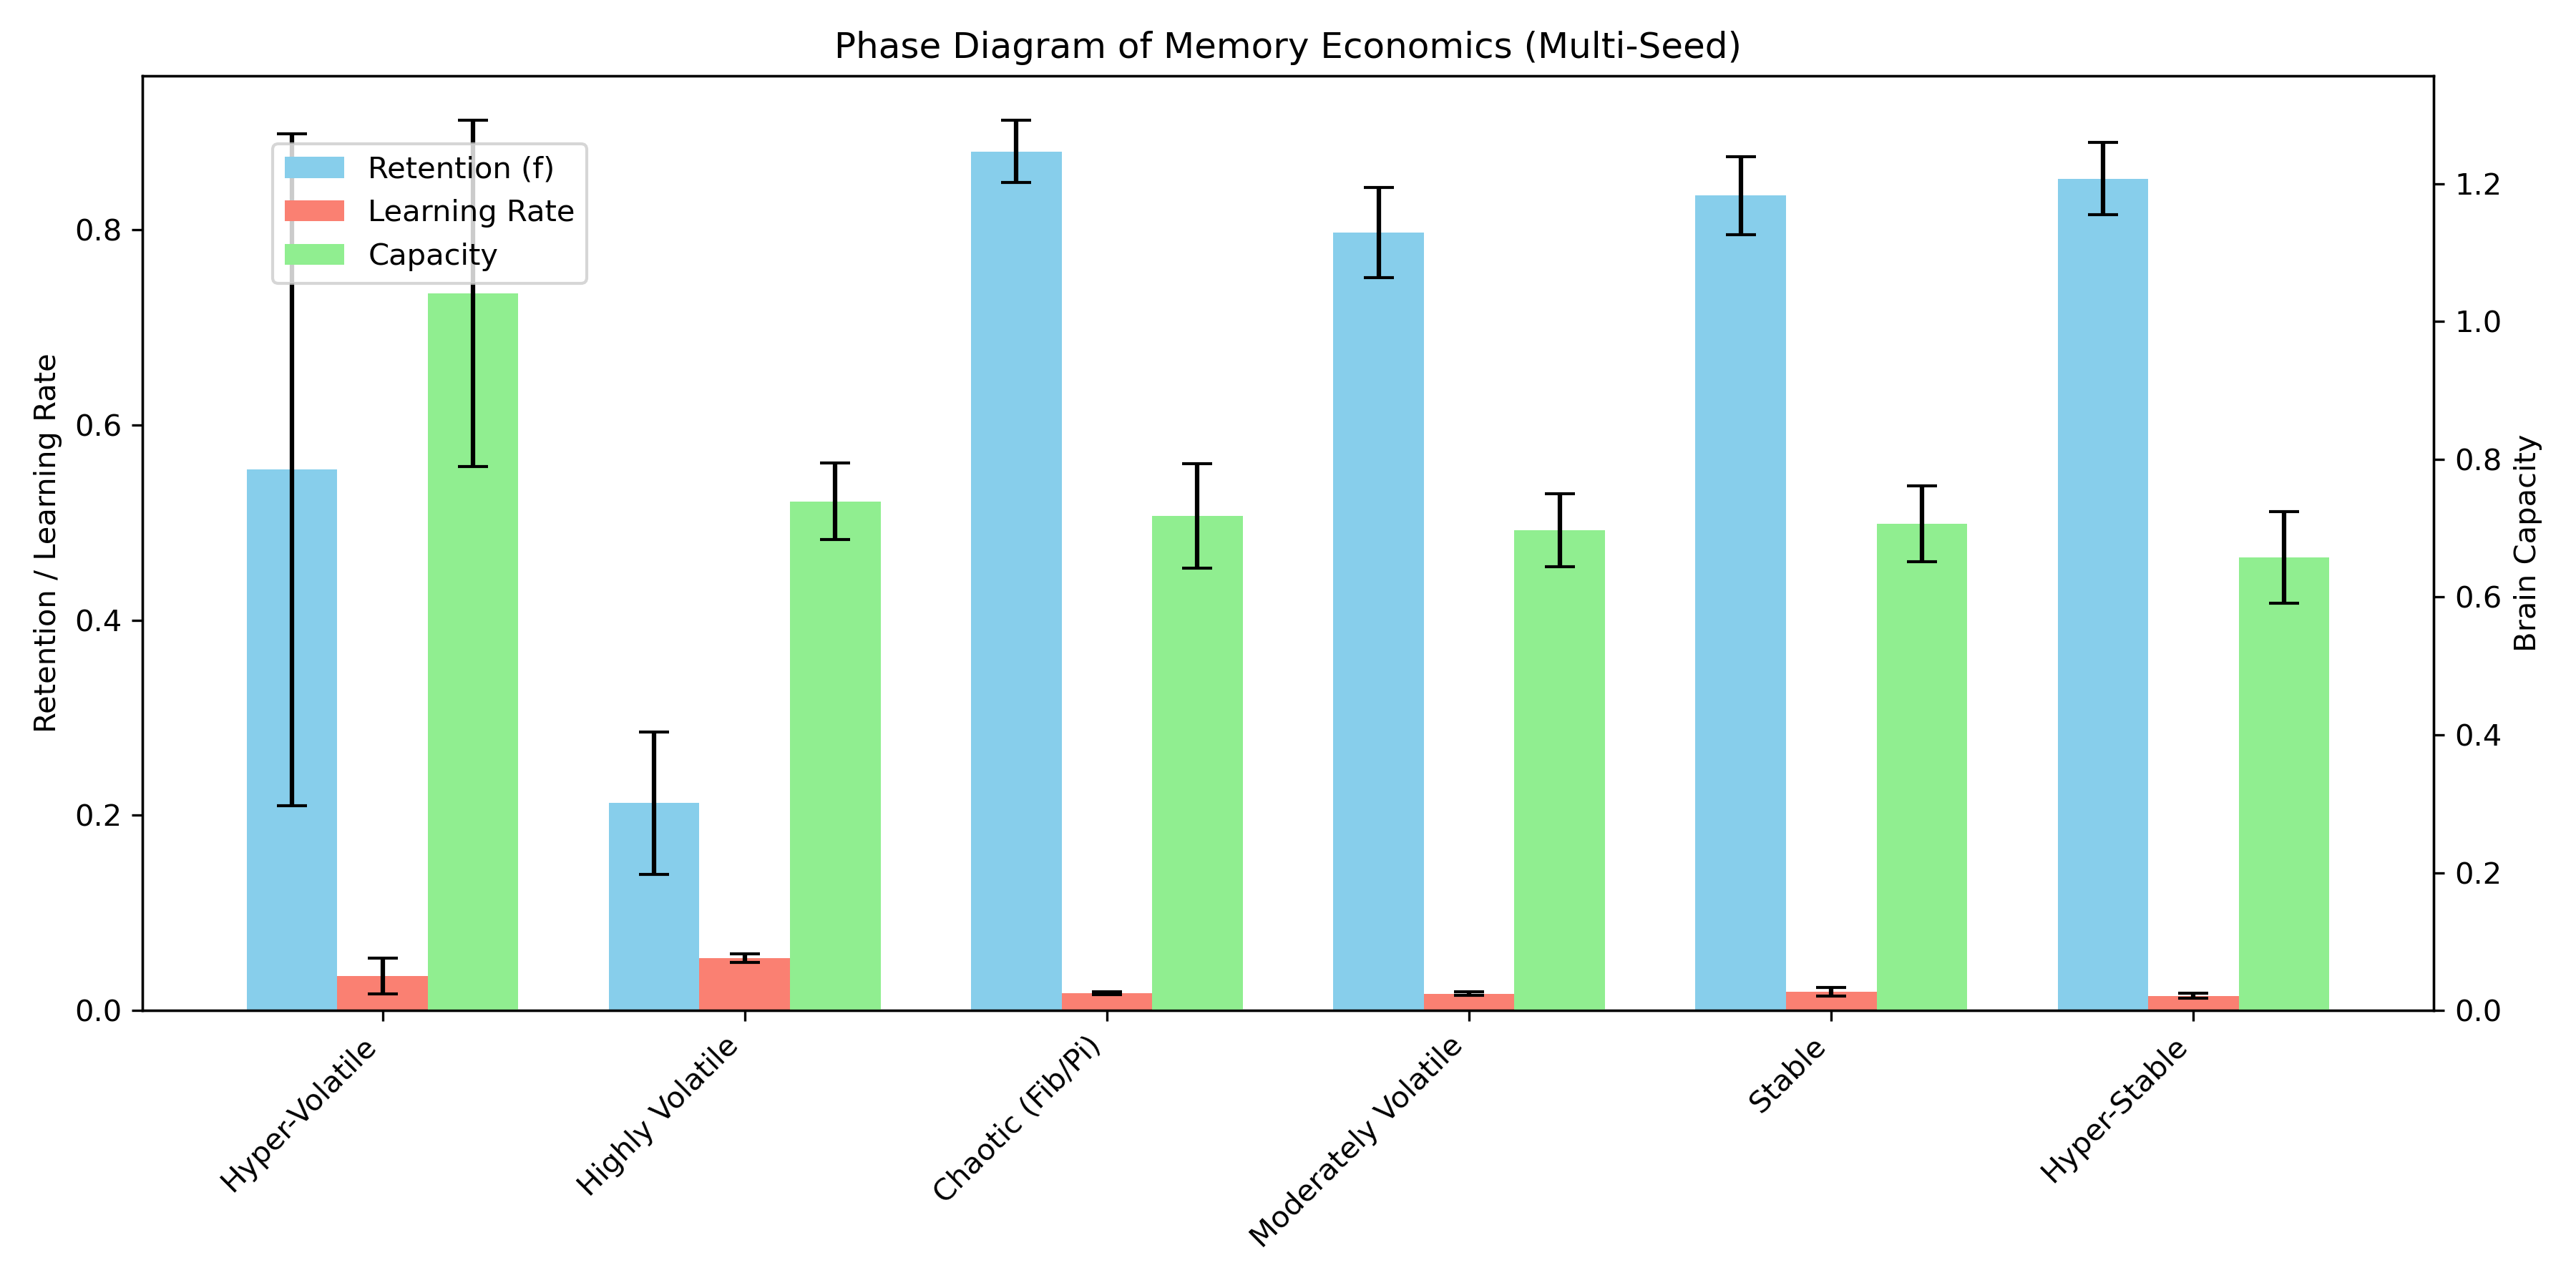
\includegraphics[width=0.92\linewidth]{figure3_phase_diagram.png}
\caption{Phase diagram of memory economics showing the non-monotonic adaptation of retention, learning rate, and capacity across environmental frequencies.}
\label{fig:phase_diagram}
\end{figure}

The evolutionary response is distinctly non-monotonic:
\begin{itemize}
    \item \textbf{The ``Boomerang'' Strategy:} At extreme volatility (shifts every 2 generations), the population preserves larger capacities ($c \approx 1.04 \pm 0.25$) and elevated retention ($f \approx 0.55 \pm 0.34$). It is metabolically cheaper to maintain enough capacity for both alternating skills than to repeatedly relearn them from scratch.
    \item \textbf{Agile Amnesia:} At intermediate volatility (shifts every 5 generations), dual-storage incurs excessive metabolic upkeep. The population crashes into low retention ($f \approx 0.21$) and high learning rates ($lr \approx 0.054$), actively wiping memory to acquire the current skill.
    \item \textbf{Lamarckian Rentiers:} During long stable periods ($\ge 20$ generations), populations converge on high retention ($f \approx 0.80 - 0.85$) and low learning rates ($lr \approx 0.015$), paying the learning cost only once per shift and surviving off inherited knowledge for the duration of the stable era.
    \item \textbf{Chaotic Hedging:} Chaotic environments select closely with the stable regime ($f \approx 0.880 \pm 0.032$), favoring robust retention to survive unpredictable shocks over the fragile agility of intermediate amnesia.
\end{itemize}

\section{Discussion}
This study provides a unified framework for understanding the economics of memory inheritance. The original observation of a fixed $\approx 0.618$ attractor is understood as a conditional state requiring slow learning, sufficient capacity, and intermediate volatility.

When agents are subject to metabolic trade-offs, inheritance strategies bifurcate. High retention is heavily favored in environments that are either highly stable (allowing skill reuse across many generations) or hyper-volatile (where skills return to relevance faster than the decay rate of memory). Agile amnesia dominates the intermediate zone where skills shift just slowly enough to make dual-storage inefficient, but fast enough to mandate constant updating.

\paragraph{Limitations.}
These results are derived from a stylized, abstract simulation. The model relies on several simplifying assumptions: agents have two explicit skill slots ($A$ and $B$); memory capacity is a scalar boundary; learning occurs via a linear additive update rule without explicit neurological interference between skills (other than capacity overflow); and fitness is calculated via a heuristic equation rather than emerging from spatial competition or complex ecology. The exact numerical values should be viewed as illustrative artifacts of these specific mathematical choices, not universal biological constants.

\paragraph{Implications.}
These findings have compelling analogies for both biology and artificial intelligence. In biology, epigenetic inheritance mechanisms should be most prominent in environments matching the ``rentier'' or ``boomerang'' timescales. In artificial intelligence, for continual learning systems operating under capacity constraints, the optimal rate of weight decay (analogous to $1 - f$) should be dynamically tuned to the spectral frequency of incoming data distributions, rather than kept as a static hyperparameter.

\end{document}
